\documentclass[12pt,letterpaper]{article}
%%%%%%%%%%%%%%%%%%%%%%%%%%%%%%
%Force pdflatex processing even with "$ latex" (required by arXiv)
\pdfoutput=1
%%%%%%%%%%%%%%%%%%%%%%%%%%%%%

\usepackage[utf8]{inputenc}
\usepackage{amsmath}
\usepackage{amssymb}
\usepackage{amsthm}
\usepackage{fp}
\usepackage{xcolor}
\definecolor{nicered}{rgb}{0.7,0.1,0.1}
\definecolor{nicegreen}{rgb}{0.1,0.5,0.1}
\usepackage[colorlinks=true,citecolor= nicegreen,linkcolor=nicered]{hyperref}
\usepackage{graphicx}
\usepackage[separate-uncertainty=true]{siunitx} 
\usepackage{cancel}

\setlength{\textwidth}{180mm}
\setlength{\oddsidemargin}{-1cm}
\setlength{\evensidemargin}{-1cm}
\setlength{\topmargin}{-1cm}

\title{Scotogenic relic density}

\author{Oscar Zapata}
\begin{document}
\maketitle

\subsection{Amplitudes}


Relic density calculation for $N_1$ as dark matter candidate. We are going to use the Mat model.

\begin{figure}
 
 	\begin{center}
    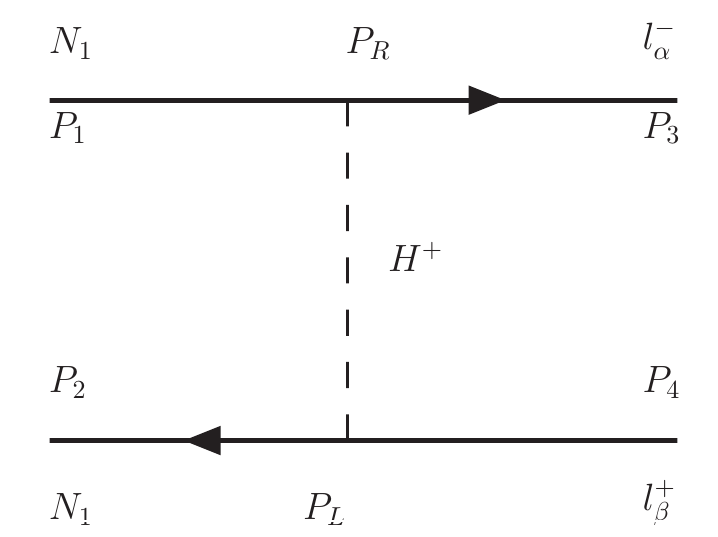
\includegraphics[scale=0.4]{1.png} 
    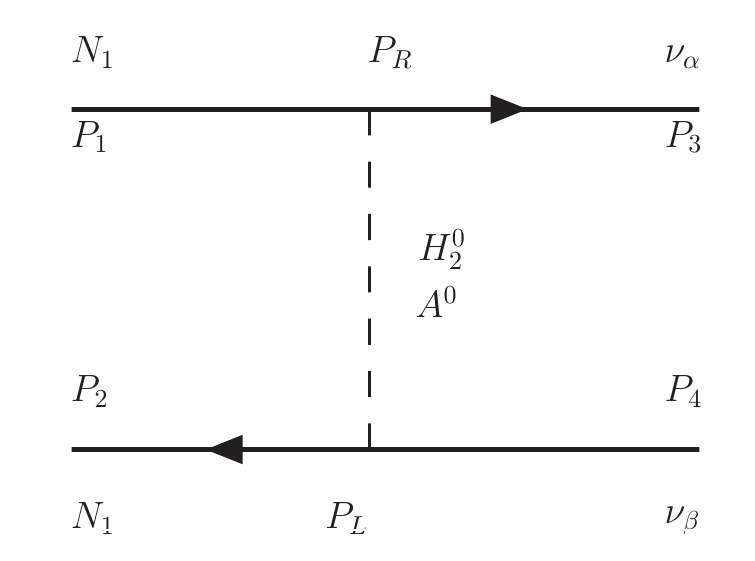
\includegraphics[scale=0.4]{2.png} \\
    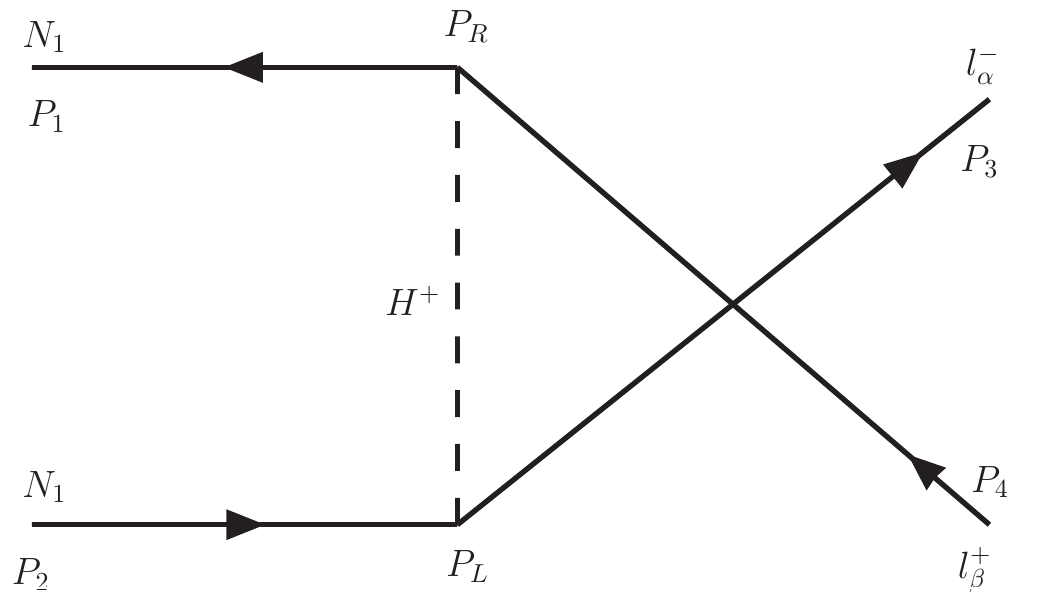
\includegraphics[scale=0.3]{3.png} 
    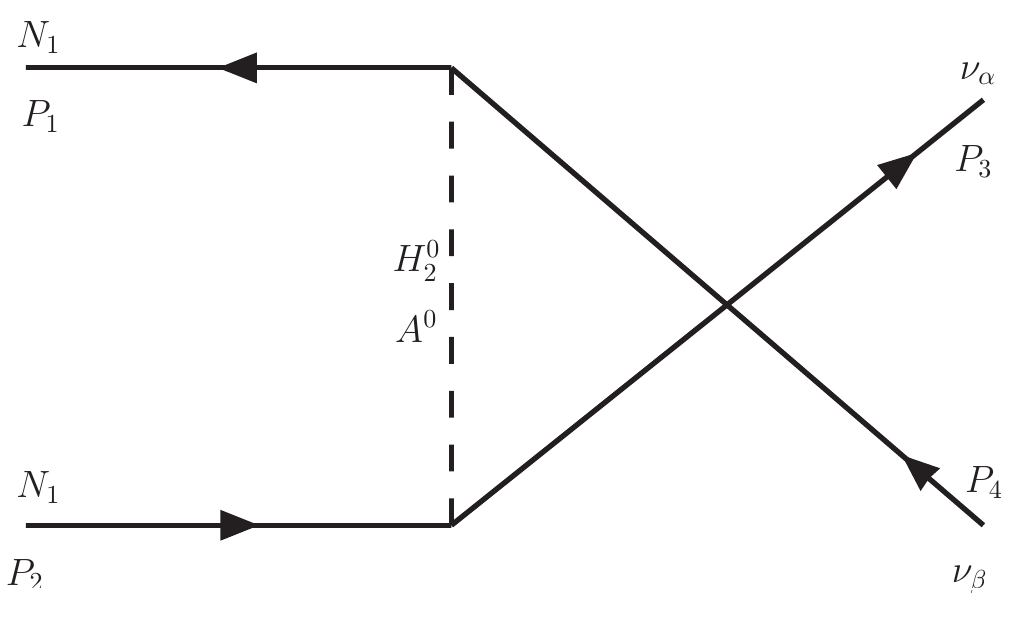
\includegraphics[scale=0.3]{4.png}
    \caption{\textbf{Diagramas de Feynman 1(a), (b), (c), (d).}}
    \label{fig:fgrd}
    \end{center}

\end{figure}

Particle content: $N_{1,2,3}$ as Majorana Fermions and
\begin{align}
  H_2=\begin{pmatrix}
    H^+\\
\frac{H^0+iA_0}{\sqrt{2}}
  \end{pmatrix}
\end{align}
The lagrangian of Yukawa is:
\begin{align}
  \mathcal{L}_Y=&Y_{\alpha i} \overline{L}_{\alpha} \widetilde{H_2} N_i+\text{h.c}\nonumber\\
=& Y_{\alpha i}\left[ \overline{\nu}_{\alpha L}\left( \frac{H^0-iA_0}{\sqrt{2}}\right) -\overline{e}_{\alpha L}H^-\right]N_i+\text{h.c}
\end{align}
We are interested in processes
\begin{align}
  N_1 N_1 \to \text{SM}\ \text{SM}
\end{align}
In order to check which vertex correspond:
\begin{align*}
  \left\langle \overline{l}l\right|\widehat{\overline{N}}\widehat{N}\left| \overline{N} N\right\rangle=
  \left\langle \overline{l}l\right|\widehat{\overline{N}}\left| \overline{N} \right\rangle=
  \left\langle \overline{l}l\right|\left. 0 \right\rangle
\end{align*}
Therefore is $P_R$ in the upper part of the diagram and $P_L$ in the down part.

%\begin{figure}
%  \centering
%  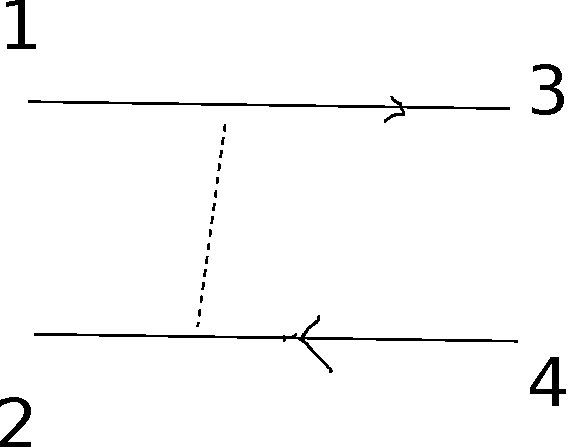
\includegraphics{ini}
%  \caption{fig }
%  \label{fig:12}
%\end{figure}

Because neutrinos do not have a defined fermion number, we have all the possibilities (Majorana Fermions Feynman Rules from Denner CERN-TH 6549/92)
\begin{align}
  N_1 N_1 & \to \nu \nu \nonumber\\
   & \to \nu \overline{\nu} \nonumber\\
   & \to \overline{\nu} \overline{\nu}
\end{align}

For the diagram 1(a). The Majorana fermions any flux of fermion number can be used. The amplitudes in the $t$ and $u$ channels are:

\begin{align}
\label{eq:tchannel}
  \mathcal{M}_t=& \left[ \overline{u}(p_3) P_R Y_{\alpha 1}u(p_1) \right]
\left[ \overline{v}(p_2) P_L Y_{\beta 1}v(p_4) \right]
\frac{1}{(q^2-m_{H^+}^2)}
\end{align}
where
\begin{align}
  q^2=(p_1-p_3)^2=(p_4-p_2)^2=t
\end{align}
\begin{align}
\label{eq:uchannel}
  \mathcal{M}_u=& \left[ \overline{u}(p_3) P_R Y_{\alpha 1}u(p_2) \right]
\left[ \overline{v}(p_1) P_L Y_{\beta 1}v(p_4) \right]
\frac{1}{(q^2-m_{H^+}^2)}
\end{align}
where
\begin{align}
  q^2=u=(p_1-p_4)^2=(p_2-p_3)^2
\end{align}

As the only difference is the interchange in final particles, we have
\begin{align*}
  \mathcal{M}=\mathcal{M}_t-\mathcal{M}_u
\end{align*}
\begin{align}
\label{eq:amplitude}
  |\mathcal{M}|^2 &= |\mathcal{M}_t|^2 + |\mathcal{M}_u|^2 - {\mathcal{M}_t}^{\dagger}\mathcal{M}_u -\mathcal{M}_t{\mathcal{M}_u}^{\dagger}\nonumber\\
                & = |\mathcal{M}_t|^2 + |\mathcal{M}_u|^2 - 2\Re(\mathcal{M}_t^{\star}\mathcal{M}_u)
\end{align}
Using the eq. ~\eqref{eq:tchannel}:
\begin{align*}
  |\mathcal{M}_{t}|^2=\frac{|Y_{\alpha 1}Y_{\beta 1}|^2}{(t-m_{H^+}^2)^2}
  \left[ \overline{v}(p_4)P_R v(p_2) \right]
  \left[ \overline{u}(p_1)P_L u(p_3) \right]
 \left[ \overline{u}(p_3)P_R u(p_1) \right]
 \left[ \overline{v}(p_2)P_L v(p_4) \right]
\end{align*}

\begin{align*}
  \frac{1}{4}\sum_{\text{spin}} |\mathcal{M}_{t}|^2=&
\operatorname{Tr}\left[ \left( \cancel{p_3}+m_3 \right)P_R (\cancel{p_1}+m_1)P_L \right]
\operatorname{Tr}\left[ \left( \cancel{p_2}-m_2 \right)P_L (\cancel{p_4}-m_4)P_R \right]
\frac{|Y_{\alpha 1} Y_{\beta 1}|^2}{(t-m_{H^+}^2)^2}\times \frac{1}{4}\\
=&\frac{1}{4}\frac{|Y_{\alpha 1} Y_{\beta 1}|^2}{(t-m_{H^+}^2)^2}
\frac{1}{2}\operatorname{Tr}\left( \cancel{p_1}\cdot\cancel{p_3} \right)
\frac{1}{2}\operatorname{Tr}\left( \cancel{p_2}\cdot\cancel{p_4} \right)\\
=&\frac{1}{4}\frac{|Y_{\alpha 1} Y_{\beta 1}|^2}{(t-m_{H^+}^2)^2}
\frac{1}{4}\left(4 p_1\cdot p_3  \right)\left(4 p_2\cdot p_4  \right)
\end{align*}
Since
\begin{align*}
 t=(p_1-p_3)^2=p_1^2+p_3^2-2p_1\cdot p_3=
m_1^2+m_{\alpha}^2-2p_1\cdot p_3 \;
\end{align*}
\begin{align*}
 t=(p_4-p_2)^2=p_4^2+p_2^2-2p_4\cdot p_2=
m_{\beta}^2+m_2^2-2p_4\cdot p_2 \;
\end{align*}
we have
\begin{align*}
  p_1\cdot p_3=\frac{m_1^2+m_{\alpha}^2-t}{2}
\end{align*}
and 
\begin{align*}
  p_2\cdot p_4=\frac{m_2^2+m_{\beta}^2-t}{2}
\end{align*}
Therefore
\begin{align*}
   \frac{1}{4}\sum_{\text{spin}} |\mathcal{M}_{t}|^2= \left\langle |\mathcal{M}|_t^2 \right\rangle
=\frac{1}{4}\frac{|Y_{\alpha 1} Y_{\beta 1}|^2}{(t-m_{H^+}^2)^2}\left( m_1^2+m_{\alpha}^2-t \right)
\left( m_2^2+m_{\beta}^2-t \right)
\end{align*}
when $m_1=m_2$ and $m_{\alpha}=m_{\beta}\to 0$
\begin{align}
\label{eq:mt2}
  \left\langle |\mathcal{M}|_t^2 \right\rangle
=\frac{1}{4}\frac{|Y_{\alpha 1} Y_{\beta 1}|^2}{(t-m_{H^+}^2)^2}\left( m_1^2-t \right)^2\,.
\end{align}

Using the eq.~\eqref{eq:uchannel}, and doing the same procedure, we have that:

%\begin{figure}
%  \centering
%  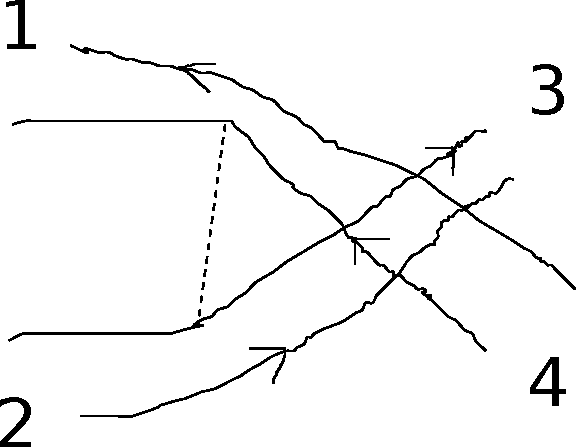
\includegraphics{fig4}
%  \caption{Fig 4}
%  \label{fig:4}
%\end{figure}

\begin{align}
\label{eq:mu2}
  \left\langle |\mathcal{M}|_u^2 \right\rangle
=\frac{1}{4}\frac{|Y_{\alpha 1} Y_{\beta 1}|^2}{(u-m_{H^+}^2)^2}\left( m_1^2-u \right)^2 .
\end{align}

Now the interference terms are:
\begin{align*}
  \mathcal{M}_t^{*} \mathcal{M}_{u}=\frac{|Y_{\alpha 1} Y_{\beta 1}|^2}{(t-m_{H^+}^2)(u-m_{H^+}^2)}
 \left[ \overline{v}(p_4) P_R v(p_2) \right]
 \left[ \overline{u}(p_1) P_L u(p_3) \right]
 \left[ \overline{u}(p_3) P_R u(p_2) \right]
 \left[ \overline{v}(P_1) P_L v(p_4) \right]
\end{align*}
By using a property of Majorana Fermions from Denner CERN-TH 6549/92:
\begin{align*}
\overline{u}(p_1,s_1)\Gamma S\Gamma\ldots \Gamma u(p_k,s_k)
=-\overline{v}(p_k,s_k) \Gamma' \ldots \Gamma' S' \Gamma' v(p_1,s_1)
\end{align*}
where
\begin{align*}
  \Gamma'=C \Gamma^T C^{-1}
\end{align*}
In particular:
\begin{align*}
  C\gamma_5 C^{-1}=-\gamma_5
\end{align*}
\begin{align}
\label{eq:cambiaespinor}
\overline{v}(p_i)P_{L,R}v(p_j)=-\overline{u}(p_j)P_{L,R}u(p_i)
\end{align}
Moreover $S'=S$ for scalar propagators. Now, using the eq.~\eqref{eq:cambiaespinor}, and the notation $u(p_j)=u_j$, we have that:
\begin{align*}
   \mathcal{M}_t^{*} \mathcal{M}_{u}=&\frac{|Y_{\alpha 1} Y_{\beta 1}|^2}{(t-m_{H^+}^2)(u-m_{H^+}^2)}
\left[- \overline{u}_2 P_R u_4 \right]
\left[ \overline{u}_3 P_L u_3 \right]
\left[ \overline{u}_3 P_R u_2 \right]
\left[ \overline{u}_4 P_L u_1 \right]\\
=&\frac{|Y_{\alpha 1} Y_{\beta 1}|^2}{(t-m_{H^+}^2)(u-m_{H^+}^2)}
\left[ \overline{u}_2 P_R u_4 \right]
\left[ \overline{u}_4 P_L u_1 \right]
\left[ \overline{u}_1 P_L u_3 \right]
\left[ \overline{u}_3 P_R u_2 \right]
\end{align*}
%correcto


\begin{align}
\dfrac{1}{4}\sum_{\text{spins}}  \overline{\mathcal{M}_t^{*} \mathcal{M}_{u}}=&\dfrac{1}{4}\frac{|Y_{\alpha 1} Y_{\beta 1}|^2}{(t-m_{H^+}^2)(u-m_{H^+}^2)}
\operatorname{Tr}\left[ \left( \cancel{p}_4+m_4 \right)P_L
\left( \cancel{p}_1+m_1 \right) P_L
\left( \cancel{p}_3+m_3 \right) P_R
\left( \cancel{p}_2+m_2 \right) P_R
\right]\nonumber\\
=&\dfrac{1}{4}\frac{|Y_{\alpha 1} Y_{\beta 1}|^2}{(t-m_{H^+}^2)(u-m_{H^+}^2)}
\operatorname{Tr}\left[ \left(m_1 \cancel{p}_4P_L + m_4m_1P_L \right)
\left( m_2\cancel{p}_3P_R+m_2m_3P_R \right) \right]\nonumber\\
=&\dfrac{1}{4}\frac{|Y_{\alpha 1} Y_{\beta 1}|^2}{(t-m_{H^+}^2)(u-m_{H^+}^2)}
\operatorname{Tr}\left[ \left(m_1m_2 \cancel{p}_4\cancel{p}_3P_R + m_4m_1m_2\cancel{p}_3P_R \right) \right]\nonumber\\
=&\dfrac{1}{4}\frac{|Y_{\alpha 1} Y_{\beta 1}|^2}{(t-m_{H^+}^2)(u-m_{H^+}^2)}
m_1m_2\operatorname{Tr}\left[ \cancel{p}_4\cancel{p}_3P_R  \right]\nonumber\\
=&\dfrac{1}{4}\frac{|Y_{\alpha 1} Y_{\beta 1}|^2}{(t-m_{H^+}^2)(u-m_{H^+}^2)}
m_1m_2 \dfrac{(4p_3\cdot p_4)}{2}
\end{align}

where we have used:
\begin{align*}
  \operatorname{Tr}\left[ \cancel{p_j}\gamma_5 \right]=0\,.
\end{align*}
\begin{align*}
  \operatorname{Tr}\left[ \cancel{p_i}\cancel{p_j}\gamma_5 \right]=0\,.
\end{align*}
\begin{align*}
  \operatorname{Tr}\left[ \cancel{p_i}\cancel{p_j}\right]
  =\operatorname{Tr}\left[ \dfrac{1}{2} \{\cancel{p_i},\cancel{p_j}\}\right]
  =\operatorname{Tr}\left[ \dfrac{1}{2} p_{i\mu}p_{j\nu}\{\gamma^{\mu},\gamma^{\nu}\}\right]
    =\operatorname{Tr}\left[ \dfrac{1}{2} p_{i\mu}p_{j\nu}2g^{\mu\nu}\right]=4p_i\cdot p_j
\end{align*}

Now using:
\begin{align}
  2 p_4\cdot p_{3}=s-\frac{m_4^2-m_3^2}{2}
\end{align}

\begin{align*}
\dfrac{1}{4}\sum_{\text{spins}}  \overline{\mathcal{M}_t^{*} \mathcal{M}_{u}}
=&\dfrac{1}{4}\frac{|Y_{\alpha 1} Y_{\beta 1}|^2}{(t-m_{H^+}^2)(u-m_{H^+}^2)}
m_1m_2 \left(s-\dfrac{m_4^2-m_3^2}{2}\right)
\end{align*}

In the limit $m_3=m_4 \rightarrow 0$ and $m_1=m_2$, we have:

\begin{align}
\label{eq:interferencia1}
\left \langle\mathcal{M}_t^{*} \mathcal{M}_{u} \right\rangle=\dfrac{1}{4}\sum_{\text{spins}}  \overline{\mathcal{M}_t^{*} \mathcal{M}_{u}}
=&\dfrac{1}{4}\frac{|Y_{\alpha 1} Y_{\beta 1}|^2}{(t-m_{H^+}^2)(u-m_{H^+}^2)}
m_1^2 s
\end{align}

In the same form:

\begin{align}
\label{eq:interferencia2}
\left \langle\mathcal{M}_u^{*} \mathcal{M}_{t} \right\rangle=\dfrac{1}{4}\sum_{\text{spins}}  \overline{\mathcal{M}_u^{*} \mathcal{M}_{t}}
=&\dfrac{1}{4}\frac{|Y_{\alpha 1} Y_{\beta 1}|^2}{(t-m_{H^+}^2)(u-m_{H^+}^2)}
m_1^2 s
\end{align}

%correcto
Therefore, using the eqs. \eqref{eq:mt2}, \eqref{eq:mu2}, \eqref{eq:interferencia1}, \eqref{eq:interferencia2} into \eqref{eq:amplitude}, we have:
\begin{align}
\label{eq:tw}
\boxed{
  \left\langle \left| \mathcal{M} \right|^2 \right\rangle=
\frac{|Y_{\alpha 1}Y_{\beta 1}|^2}{4} \left\{ 
\frac{\left(m_1-t  \right)^2}{\left( m_{H^+}^2-t \right)^2}+
\frac{\left(m_1-u  \right)^2}{\left( m_{H^+}^2-u \right)^2}-
\frac{2 m_1^2 s}{\left( t-m_{H^+}^2 \right)\left( u-m_{H^+}^2 \right)}
 \right\}
 }
\end{align}

The results should be the same for $N_1 N_1 \to \overline{\nu}_\alpha \nu_\beta$ but mediated by $H^0$ and $A^0$.
The combined result for $H^0$ and $A^0$ should give the same contribution of the charged Higgs.

The contributions with Lepton number violation $\nu\nu$ and
$\overline{\nu}\overline{\nu}$ is proportional to neutrino masses and
are in general negligible.

In this way, the total width is just a factor 2 of \eqref{eq:tw}.

\begin{figure}
  \centering
  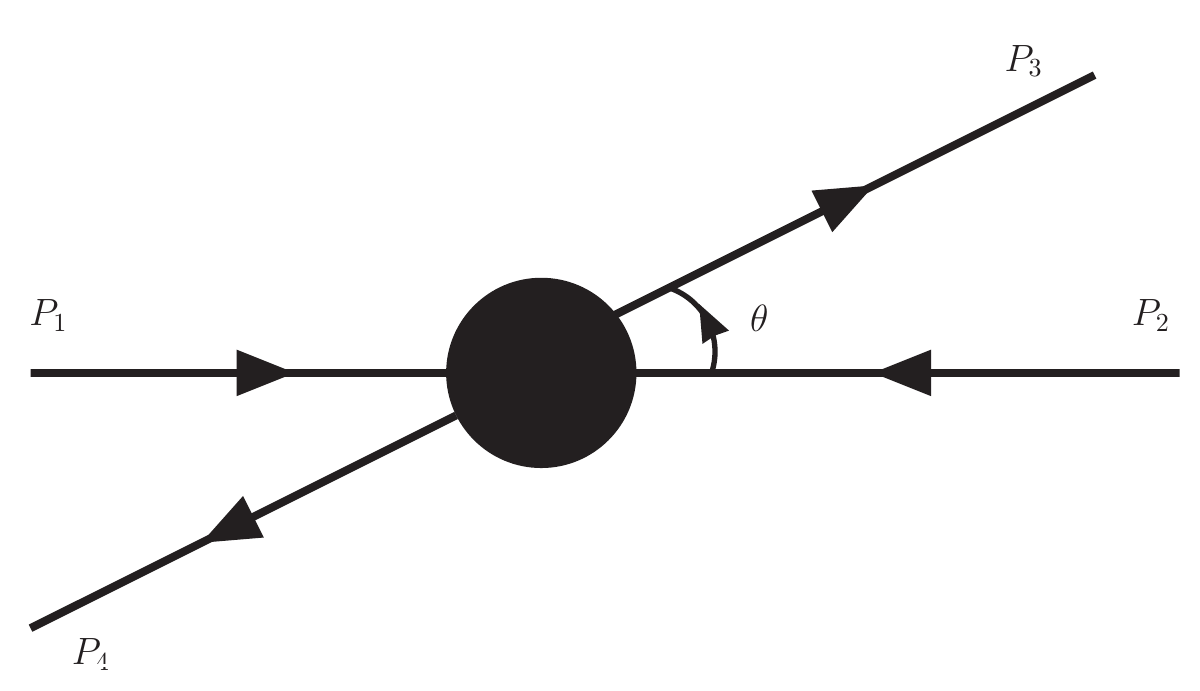
\includegraphics[scale=0.3]{angulo.png}
  \caption{Colisión en el centro de masa CM}
  \label{fig:g}
\end{figure}

Now, we know that:

\begin{align*}
  p_i=&(E_i,\mathbf{p}_i)\\
  p_i^2=&m_i^2
\end{align*}
therefore:
\begin{align}
  t=&(p_1-p_3)^2  = p_1^2+p_3^2-2p_1\cdot p_3\nonumber\\
=& m_1^2+m_3^2-2(E_1 E_3-|\mathbf{p}_1||\mathbf{p}_3|\cos\theta)\nonumber\\
\approx & m_1^2+m_3^2-2(E_1 E_3-|\mathbf{p}_1|E_3\cos\theta)\nonumber\\
=& m_1^2+m_3^2-2(E_1 E_1-|\mathbf{p}_1|E_1\cos\theta)
\end{align}

where $\theta$ is the angle showed in the Figure ~\ref{fig:g}. In general we have the \textbf{Mandelstam variables}:

\begin{align}
\label{eq:mandelstam}
  s=& \left(E_1+E_2\right)^2=\left(E_3+E_4\right)^2=4E_1^2\nonumber\\
t\approx &  m_1^2-2E_1^2+2E_1|\mathbf{p}_1|\cos(\theta)\nonumber\\
u\approx & 2m_1^2 -t -s
\end{align}

in the last equation we used the known relation $s+t+u=m_1^2+m_2^2+m_3^2+m_4^2 $.

Using:
\begin{align}
  |\mathbf{p}_1|=m_1v_1
\end{align}
\begin{align*}
  v_{\text{rel}}=v_1-v_2=2v_1 \Rightarrow   v_1=\frac{v_{\text{rel}}}{2} ,
\end{align*}
\begin{align}
\label{eq:p1}
  |\mathbf{p}_1|=m_1 \frac{v_{\text{rel}}}{2}
\end{align}
\begin{align}
\label{eq:energy}
  E_1=E_2=\sqrt{m_1^2+m_1^2 \frac{v_{\text{rel}}^2}{4}}
\end{align}

Now, the differential cross for $2\to 2$ is:

\begin{align}
  \frac{d\sigma}{d\Omega}=&\frac{1}{64\pi^2 s}
\left[ \frac{\left(s-(\cancel{m_3+m_4})^2  \right)\left(s-(\cancel{m_3-m_4})^2  \right)}{\left(s-(m_1+m_2)^2  \right)\left(s-(\cancel{m_1-m_2})^2  \right)} \right]\left\langle |\mathcal{M}|^2 \right\rangle\nonumber\\
=&\frac{1}{64\pi^2 s}\frac{1}{\left( 1-4 m_1^2/s \right)^{1/2}}
\left\langle |\mathcal{M}|^2 \right\rangle
\end{align}

\begin{align}
  \frac{d\sigma}{d\Omega}
=&\frac{1}{64\pi^2 s}\frac{|\mathbf{p}_f|}{|\mathbf{p}_{i}|}\left\langle |\mathcal{M}|^2 \right\rangle 
\end{align}

which is the eq. 4.35 of Halzen F. Martin A.D., Quarks and Leptons book.\\

now 

\begin{align}
  \frac{d\sigma}{d\Omega}
=&\frac{1}{64\pi^2 s}\frac{E_1}{m_1 \frac{v_{\text{rel}}}{2}}\left\langle |\mathcal{M}|^2 \right\rangle 
\end{align}

using the eqs.~\eqref{eq:tw},  ~\eqref{eq:p1},


\begin{align}
  \frac{d\sigma}{d\Omega}=&\frac{1}{64\pi^2 s m_1 \frac{v_{\text{rel}}}{2}}E_1 \times \frac{|Y_{\alpha 1}Y_{\beta 1}|^2}{4} \left\{ 
\frac{\left(m_1-t  \right)^2}{\left( m_{H^+}^2-t \right)^2}+
\frac{\left(m_1-u  \right)^2}{\left( m_{H^+}^2-u \right)^2}-
\frac{2 m_1^2 s}{\left( t-m_{H^+}^2 \right)\left( u-m_{H^+}^2 \right)}
 \right\}
\end{align}

using the eq.~\eqref{eq:energy} and eq.~\eqref{eq:mandelstam} for the energi $E_1$ and the Mandelstam variables and using Mathematica, we can calculate the expansion $ \langle \sigma v \rangle =a+bv^2+ \cdots$

we obtain: 

\begin{align}
\langle \sigma v \rangle \approx \dfrac{m_1^2(m_1^4+m_{H^+}^4)}{48\pi(m_1^2+m_{H^+}^2)}v_{\text{rel}}^2 + O(v^4)
\end{align}

we had obtain $a=0$, $b\neq 0$. 

 \subsection{Boltzman equation}

\begin{align*}
  \frac{dy}{dt}=\sqrt{\frac{\pi}{45}}g_{*}^{1/2}M_p \left\langle \sigma_{\text{eff}}v \right\rangle
  \left( y^2-y_{\text{eq}}^2 \right)
\end{align*}
See Gellmini and Gondolo et al paper.
\begin{align*}
  \Omega h^2=\frac{\rho h^2}{\rho_c}=\frac{m_1 n_1}{\rho_c}h^2=\frac{m_1 y^0_1 s^0}{\rho_c}
\end{align*}
where
\begin{align*}
  \rho_c=\frac{3H^2}{8\pi G}=1.05 h^2\times 10^{-3} \text{GeV/cm${}^{3}$}
\end{align*}
\begin{align*}
  s^0=\frac{g_s(T^0)2\pi^2}{45}T_0^3=\SI{2892.45}{cm^{-3}}
\end{align*}
\begin{align*}
  T_0=\SI{2.726}{K}
\end{align*}
\begin{align*}
  g_s(T_0)=3.913
\end{align*}
and finally
\begin{align*}
  \Omega h^2=2.75\times 10^8 \frac{m_1}{\text{GeV}} y_1^0
\end{align*}


\begin{align*}
  \frac{1}{y_0}=\frac{1}{y_{\text{f.o}}}-\sqrt{\frac{\pi}{45}}M_p\int_{T_{\text{f.o}}}^{T_0}
   g_{*}^{1/2} \left\langle \sigma v \right\rangle dT
\end{align*}
\begin{align*}
  y_0=\frac{\sqrt{45/\pi}}{m_1 M_p g_{*}^{1/2} J(x_{\text{f.o}})}
\end{align*}
where
\begin{align*}
  J(x_{\text{f.o}}=\int_{x_{\text{f.o}}}^{x_0} \frac{\left\langle  \sigma v\right\rangle}{x^2}dx
\end{align*}
where
\begin{align*}
  x=\frac{m}{T}
\end{align*}


\begin{align*}
  \left\langle \sigma v \right\rangle
=a+6 \left( b-\frac{a}{4} \right)\frac{1}{x}\approx=a+\frac{6b}{x}
\end{align*}

\begin{align*}
  y(x_f)=&\frac{3b}{x_f^2}+a \left(x_f-\frac{3}{4}  \right)\frac{1}{x_f^2}\\
=&\left[ a+3 \left( b-\frac{a}{4} \right) \right]\frac{1}{x_f}\\
\approx & \left( a+\frac{3b}{x_f} \right)\frac{1}{x_f}
\end{align*}

\begin{align*}
  \Delta=y-y_{\text{eq}}
\end{align*}

\begin{align*}
  \frac{d\Delta}{dx}=-\sqrt{\frac{\pi}{45}}\frac{M_P g_{*}^{1/2}m_1 \left\langle \sigma v \right\rangle}{x^2}
\Delta \left( \Delta +2y_{\text{eq}} \right)-\frac{dy_{\text{eq}}}{dx}
\end{align*}
before decoupling
\begin{align*}
  y=(1+\delta)y_{\text{eq}}
\end{align*}
\begin{align*}
  \Delta=\delta y_{\text{eq}} 
\end{align*}
and
\begin{align*}
  \frac{d\Delta}{dx}=0
\end{align*}
\begin{align*}
  -\frac{\pi}{45} \frac{M_p g_{*}^{1/2}m_1}{x^2}\left\langle \sigma v \right\rangle \delta(\delta+2)y_{\text{eq}}
=\frac{1}{y_{\text{eq}}}\frac{d y_{\text{eq}}}{dx}
\end{align*}
\begin{align*}
  y_{\text{eq}}\sim x^{3/2}e^{-x}
\end{align*}
\begin{align*}
  -\frac{\pi}{45} \frac{M_p g_{*}^{1/2}m_1}{x^2}\left\langle \sigma v \right\rangle \delta(\delta+2)
\frac{g_1 x^{3/2} e^{-x}}{g_S 2^{5/2}\pi^{3/2}/45}=
\frac{(1-(3/2)x)e^{-x}x^{3/2}}{x^{3/2}e^{-x}}
\end{align*}
\begin{align*}
  e^{x_f}=\frac{0.0382 M_P m_1 \left\langle \sigma v \right\rangle}{g_{*}^{1/2}x_f^{1/2}}
\end{align*}

\end{document}
